% Pengaturan ukuran teks dan bentuk halaman dua sisi
\documentclass[10pt,twoside]{report}

% Pengaturan ukuran halaman dan margin
\usepackage[a5paper,top=25mm,left=25mm,right=20mm,bottom=25mm]{geometry}

% Mnecegah meregangkan paragraf untuk meratakan bawah halaman
\raggedbottom

% Pengaturan ukuran spasi
\usepackage[singlespacing]{setspace}

% Font Times New Roman
%\usepackage{mathptmx}

% Gunakan T1 font encoding terbaru untuk texlive 2025
\usepackage[T1]{fontenc}

% Gunakan package untuk fonts
% NOTE: Gunakan Compiler XeLaTex atau LuaLaTex karena default 
% pdflatex tidak mendukung fontspec
\usepackage{fontspec}

% Gunakan font Trebuchet
%\usepackage{trebuchet}

% Prevent table overflow
\usepackage{tabularx}

% Pengaturan gambar 
\usepackage{float}

% Judul dokumen
\title{Buku Laporan Kerja Praktik ITS}
\author{Alief Gilang Permana Putra}

% Pengaturan format bahasa
\usepackage[indonesian]{babel}

% Pengaturan jenis karakter
\usepackage[utf8]{inputenc}

\usepackage[final]{microtype}

% Pengaturan ukuran indentasi paragraf
\setlength{\parindent}{2em}

% Pengaturan ukuran spasi paragraf
\setlength{\parskip}{0.5ex}

% Package lainnya
\usepackage{etoolbox} % Mengubah fungsi default
\usepackage{enumitem} % Pembuatan list
\usepackage{lipsum} % Pembuatan template kalimat
\usepackage{graphicx} % Input gambar
\usepackage{longtable} % Pembuatan tabel
\usepackage[table,xcdraw]{xcolor} % Pewarnaan tabel
\usepackage[numbers, sort&compress, square]{natbib} % Kutipan artikel menggunakan angka
%\usepackage{natbib} % Kutipan artikel
\usepackage{eso-pic} % Pembuatan background
\usepackage{changepage} % Pembuatan teks kolom
\usepackage{wrapfig} % Wrapping gambar

\usepackage{amsmath}

%% Gunakan opsi [titles] agar format Judul "DAFTAR ISI" tidak berubah
%\usepackage[titles]{tocloft}
%
%% Atur jarak vertikal antar Bab di Daftar Isi
%% Ubah 0pt sesuai selera (0pt = sangat rapat, 5pt = agak renggang)
%\setlength{\cftbeforechapskip}{5pt}

% Pengaturan detail pada file PDF
\usepackage[pdfauthor={\@author},bookmarksnumbered,pdfborder={0 0 0}]{hyperref}

% Definisi untuk "Halaman ini sengaja dikosongkan"
\def\kosong{
  \begin{center}\textit{Halaman ini sengaja dikosongkan}\end{center}
}

% Definisi baru yang lebih baik untuk "Halaman ini sengaja dikosongkan"
\newcommand{\halamankosong}{
	\newpage
	\thispagestyle{fancy}
	\begin{center}
		\textit{Halaman ini sengaja dikosongkan}
	\end{center}
	\clearpage
}
\patchcmd{\cleardoublepage}{\hbox{}}{\halamankosong}{}{}


% Pengaturan penomoran halaman
\usepackage{fancyhdr}
\fancyhf{}
\renewcommand{\headrulewidth}{0pt}
\pagestyle{fancy}
\fancyfoot[CE,CO]{\thepage}
\patchcmd{\chapter}{plain}{fancy}{}{}
\patchcmd{\chapter}{empty}{plain}{}{}

% Pengaturan format judul bab
\usepackage{titlesec}
\titleformat{\chapter}[display]{\bfseries\Large}{BAB \centering\Roman{chapter}}{0ex}{\vspace{0ex}\centering}[\vspace{2ex}]
\titleformat{\section}{\bfseries\large}{\MakeUppercase{\thesection}}{1ex}{}
\titleformat{\subsection}{\bfseries\large}{\MakeUppercase{\thesubsection}}{1ex}{}
\titleformat{\subsubsection}{\bfseries\large}{\MakeUppercase{\thesubsubsection.}}{1ex}{}
\titlespacing{\chapter}{0ex}{0ex}{2ex}
\titlespacing{\section}{0ex}{1ex}{1ex}
\titlespacing{\subsection}{0ex}{1ex}{0.5ex}
\titlespacing{\subsubsection}{1em}{1ex}{0.5ex}
% Set kedalaman penomoran
\setcounter{secnumdepth}{3}

% Set penomoran subsubsection menjadi alphabetic
\renewcommand{\thesubsubsection}{\Alph{subsubsection}}
\usepackage{notoccite}

% Pengaturan persamaan
\newenvironment{conditions}
{\par\vspace{\abovedisplayskip}\noindent
  \tabularx{\columnwidth}{>{$}l<{$} @{${}={}$} >{\raggedright\arraybackslash}X}}
{\endtabularx\par\vspace{\belowdisplayskip}}

% Pengaturan format baris program
\usepackage{listings}
\definecolor{comment}{RGB}{0,128,0}
\definecolor{string}{RGB}{255,0,0}
\definecolor{keyword}{RGB}{0,0,255}
\lstdefinestyle{codestyle}{
  commentstyle=\color{comment},
  stringstyle=\color{string},
  keywordstyle=\color{keyword},
  basicstyle=\footnotesize\ttfamily,
  numbers=left,
  numberstyle=\tiny,
  numbersep=5pt,
  frame=lines,
  breaklines=true,
  prebreak=\raisebox{0ex}[0ex][0ex]{\ensuremath{\hookleftarrow}},
  showstringspaces=false,
  upquote=true,
  tabsize=2,
  captionpos=b,
}
\lstset{style=codestyle}

% Mengganti figure dan table menjadi gambar dan tabel
\renewcommand{\figurename}{Gambar}
\renewcommand{\tablename}{Tabel}
\renewcommand{\lstlistingname}{Kode Sumber}
% Isi keseluruhan dokumen
\begin{document}
  % Gunakan font Times New Roman
  \setmainfont{Times New Roman}
  % Nomor halaman pembuka dimulai dari sini
  \pagenumbering{gobble}

  % Sampul luar
  {
  	\setmainfont{Trebuchet MS}\color{white}
  	\input{sampul/sampul-luar.tex}
  	
  }
  

  % Sampul dalam
  {
  	\setmainfont{Trebuchet MS}
  	\AddToShipoutPictureBG*{
  \AtPageLowerLeft{
    % Ubah nilai berikut jika posisi horizontal background tidak sesuai
    \hspace{-3.5mm}

    % Ubah nilai berikut jika posisi vertikal background tidak sesuai
    \raisebox{0mm}{
      
\includegraphics[width=\paperwidth,height=\paperheight]{sampul/sampul-dalam.png}
    }
  }
}

% Pengaturan margin untuk menyesuaikan konten sampul
\newgeometry{top=70mm,left=25mm,right=20mm,bottom=25mm}

\begin{flushleft}

  % Pengaturan jenis teks yang digunakan
  \sffamily

  % Ubah penomoran buku berikut sesuai dengan yang ditentukan oleh departemen
  \noindent\textbf{KERJA PRAKTIK - EF234603}
  \vspace{4ex}

  % Ubah kalimat berikut sesuai dengan judul topik kerja praktik
  \noindent{\Large \textbf{MEDICAL IMAGE CAPTIONING}} \\
  \vspace{4ex}
  
  % Ubah kalimat berikut sesuai dengan nama tempat kerja praktik
  \noindent{\large \textbf{Laboratorium Manajemen Cerdas Informasi}}
  %\vspace{2ex}
  
  % Ubah kalimat berikut sesuai dengan alamat tempat kerja praktik
  \noindent{\normalsize{Jalan Teknik Kimia - Gedung Departemen Teknik Informatika, \\ Kampus Institut Teknologi Sepuluh Nopember \\ Jalan Raya ITS, Sukolilo, Surabaya 60111, Indonesia}}
  \vspace{2ex}
  
  % Ubah tanggal berikut sesuai dengan waktu berlangsungnya kerja praktik
  \noindent{\textbf{Periode:} \normalsize{27 Mei 2025 - 27 Agustus 2025}}
  \vspace{2ex}
  
  \begin{adjustwidth}{-2mm}{}
  	\begin{tabular}{lcp{0.7\linewidth}}
  		% Ubah kalimat-kalimat berikut sesuai dengan nama dan NRP mahasiswa pertama
  		\textbf{Oleh:} & & \\
  		\normalsize{Alief Gilang Permana Putra} & & \normalsize{ 5025221193} \\
  		% Ubah kalimat-kalimat berikut sesuai dengan nama dan NRP mahasiswa kedua
  		%\textbf{Felix Arvid Ulf Kjellberg} & & \textbf{NRP 0123 20 4000 0002} \\
  		
  	\end{tabular}
  \end{adjustwidth}
  \vspace{4ex}
  
  \noindent\textbf{Pembimbing Jurusan} \\
  % Ubah kalimat berikut sesuai dengan nama dosen pembimbing
  \normalsize{Shintami Chusnul Hidayati, S.Kom., M.Sc., Ph.D.}
  %\vspace{10ex}
  \vspace{2ex}
  
  \noindent\textbf{Pembimbing Lapangan} \\
  % Ubah kalimat berikut sesuai dengan nama dosen pembimbing
  \normalsize{Dr. Kelly Rossa Sungkono, S.Kom., M.Kom.}
  \vspace{3ex}
  
  % Ubah kalimat berikut sesuai dengan nama departemen
  \noindent\textbf{DEPARTEMEN TEKNIK INFORMATIKA} \\
  % Ubah kalimat berikut sesuai dengan nama fakultas
  \textbf{Fakultas Teknologi Elektro dan Informatika Cerdas} \\
  \textbf{Institut Teknologi Sepuluh Nopember} \\
  % Ubah kalimat berikut sesuai dengan tempat dan tahun pembuatan buku
  \textbf{Surabaya 2025}

\end{flushleft}

\restoregeometry

%  	\cleardoublepage
  }
  
  \halamankosong
  
  \pagenumbering{roman}
   % Daftar isi
  \renewcommand*\contentsname{DAFTAR ISI}
  \phantomsection
  \addcontentsline{toc}{chapter}{\contentsname}
  \tableofcontents
  \cleardoublepage
  
  % Lembar pengesahan untuk perusahaan
  %\input{pengesahan/pengesahan-perusahaan.tex}
  %\cleardoublepage

  % Daftar gambar
  \renewcommand*\listfigurename{DAFTAR GAMBAR}
  \phantomsection
  \addcontentsline{toc}{chapter}{\listfigurename}
  \listoffigures
  \cleardoublepage

  % Daftar tabel
  \renewcommand*\listtablename{DAFTAR TABEL}
  \phantomsection
  \addcontentsline{toc}{chapter}{\listtablename}
  \listoftables
  \cleardoublepage
  
  % Daftar kode
  \renewcommand*\lstlistlistingname{DAFTAR KODE SUMBER}
  \lstlistoflistings
  \addcontentsline{toc}{chapter}{\lstlistlistingname}
  \cleardoublepage
  
  % Lembar pengesahaan untuk departemen
  \phantomsection
  \addcontentsline{toc}{chapter}{LEMBAR PENGESAHAN}

\begin{center}
  {\Large \textbf{LEMBAR PENGESAHAN}} \\
  \vspace{1ex}
  {\large \textbf{KERJA PRAKTIK}}
  \vspace{6ex}

  % Ubah kalimat berikut sesuai dengan judul topik kerja praktik
  {\Large \textbf{MEDICAL IMAGE CAPTIONING}}
  \vspace{6ex}
  
  \large{Oleh:}
  \vspace{1ex}
  
  \begin{tabular}{l @{\hspace{1cm}} l}
  	\large{Alief Gilang Permana Putra} & \large{5025221193}
  \end{tabular}
  \vspace{6ex}
  
  %Disetujui oleh Pembimbing Kerja Praktik:
  \vspace{4ex}

\end{center}

\noindent % Prevent indentation of the entire line
%
% Minipage for the left signature block
\begin{minipage}[t]{0.35\textwidth}
	\centering
	Mengetahui, \\[2ex]
	Dosen Pembimbing Kerja Praktik \\[4ex] % More space for signature
	%\includegraphics[width=4cm]{signature1.png} \\[2ex]
	\textbf{Shintami Chusnul Hidayati, S.Kom., M.Sc., Ph.D.} \\
	NIP. 1994201912088
\end{minipage}
%
\hfill % Pushes the two blocks apart to the edges
%
% Minipage for the right signature block
\begin{minipage}[t]{0.35\textwidth}
	\centering
	Menyetujui, \\[2ex]
	Pembimbing Lapangan Kerja Praktik \\[4ex] % More space for signature
	%\includegraphics[width=4cm]{signature2.png} \\[2ex]
	\textbf{Dr. Kelly Rossa Sungkono, S.Kom., M.Kom.} \\
	NIP. 1987202012004
\end{minipage}


  \cleardoublepage
  
  % Abstrak
  \phantomsection
  % Main title
\begin{center}
	\large{\textbf{PENGEMBANGAN MODUL KOREKSI DAN KLASIFIKASI ARTEFAK CITRA SEBAGAI BAGIAN DARI SISTEM FAULT TOLERANCE IMAGE CAPTIONING}}
\end{center}
\vspace{1ex}

%\vspace{1.5cm} % Add vertical space after the title

% --- INFO BLOCK ---
% Use a tabular environment for perfectly aligned columns.
% The @{} syntax precisely controls the spacing around the colons.
\noindent
% The width of the last column was reduced to fit on A5 paper
\begin{tabular}{l @{\hspace{2mm}} l @{\hspace{5mm}} p{0.55\textwidth}} %<-- Reduced width
	Nama Mahasiswa & : & Alief Gilang Permana Putra\\
	NRP & : & 5025221193 \\
	Departemen & : & Teknik Informatika - FTEIC \\
	Pembimbing Departemen & : & Shintami Chusnul Hidayati, S.Kom., M.Sc., Ph.D. \\
	Pembimbing Lapangan & : & Dr. Kelly Rossa Sungkono, S.Kom., M.Kom \\[4ex]
\end{tabular}

\vspace{2ex} % Vertical space before the abstract

% --- ABSTRAK ---
\begin{center}
	{\textbf{ABSTRAK}}
\end{center}

% The abstract paragraph
Ini Abstrak \lipsum[1][1-10]

\vspace{2ex} % Vertical space before keywords

% --- KATA KUNCI ---
\noindent\textbf{Kata Kunci :} Kata kunci


  \cleardoublepage
  
  % Kata pengantar
  \phantomsection
  \addcontentsline{toc}{chapter}{KATA PENGANTAR}

\begin{center}
  \Large\textbf{KATA PENGANTAR}
\end{center}
\vspace{2ex}

% Ubah paragraf-paragraf berikut sesuai dengan yang ingin diisi pada kata pengantar

Puji dan syukur ke hadirat Allah SWT atas segala rahmat, hidayah, dan karunia -Nya sehingga penulis dapat menyelesaikan salah satu kewajiban sebagai mahasiswa departemen teknik informatika, yaitu kerja praktik dengan judul "PENGEMBANGAN MODUL KOREKSI DAN KLASIFIKASI ARTEFAK CITRA OTAK SEBAGAI BAGIAN DARI SISTEM \textit{FAULT TOLERANCE IMAGE CAPTIONING}" di Laboratorium Manajemen Cerdas Informasi.

Penulis menyadari masih banyak kekurangan baik dalam pelaksanaan kerja praktik maupun penyusunan buku laporan ini. Namun penulis berharap buku laporan ini dapat menjadi refleksi dan evaluasi bagi penulis serta dapat menambah wawasan pembaca dan menjadi sumber referensi.

Melalui buku ini, penulis mengucapkan terima kasih kepada orang-orang yang telah membantu dan memberikan dukungan dalam penyusunan laporan kerja praktik ini, baik secara langsung maupun tidak langsung kepada:

\begin{enumerate}[nolistsep]

  \item Kedua orang tua penulis.

  \item Ibu Shintami Chusnul Hidayati, S.Kom, M.Sc., Ph.D, selaku dosen pembimbing kerja praktik. 

  \item Ibu Dr. Kelly Rossa Sungkono, S.Kom., M.Kom., selaku pembimbing lapangan kerja praktik.
  
  \item Mas Ibad dan Mbak Sabrina, yang telah membantu dan membimbing penulis dalam melaksanakan kerja praktik.

\end{enumerate}


\begin{flushright}
  \begin{tabular}[b]{c}
    % Ubah kalimat berikut sesuai dengan tempat, bulan, dan tahun penulisan
    Surabaya, Agustus 2025
    \\
    \\
    \\
    \\
    Alief Gilang Permana Putra
  \end{tabular}
\end{flushright}

  \cleardoublepage

  % Nomor halaman isi dimulai dari sini
  \pagenumbering{arabic}

  % Bab 1 pendahuluan
  % Ubah kalimat sesuai dengan judul dari bab ini
\chapter{PENDAHULUAN}

% Ubah konten-konten berikut sesuai dengan yang ingin diisi pada bab ini

\section{Latar Belakang}

\textit{Magnetic Resonance Imaging} (MRI) merupakan salah satu teknologi pencitraan medis non invasif yang digunakan untuk melakukan visualisasi struktur otak secara detail dengan kemampuan yang dapat menghasilkan kontras jaringan lunak yang tinggi dan resolusi spasial yang baik \citep{Safari2024}. Citra MRI otak digunakan secara luas dalam diagnosis, penelitian neurologi, dan pengembangan sistem berbasis \textit{Artificial Intelligence} (AI) seperti deteksi, segmentasi, klasifikasi, dan \textit{image captioning} \citep{Liu2018}. MRI juga digunakan untuk menghasilkan citra dengan resolusi tinggi yang mendukung diagnosis penyakit otak seperti tumor dan stroke serta membantu dalam perencanaan terapi \citep{Zhuge2017,Assam2021}. 

Salah satu tantangan utama dalam akuisisi citra MRI adalah munculnya artefak terutama akibat pergerakan pasien selama proses pemindaian yang memakan waktu lama. Artefak ini dapat menurunkan kualitas citra, mengganggu analisis lanjutan, bahkan menyebabkan salah diagnosis atau perlunya pengulangan pemindaian \citep{Safari2024}. Artefak juga berdampak signifikan pada akurasi diagnostik manusia maupun sistem berbasis AI \citep{Krag2025}. Artefak pada MRI otak dapat diklasifikasikan berdasarkan sumber dan bentuknya. Salah satu jenis yang paling umum adalah \textit{motion artifact}, yang dapat berupa translasi (gerakan vertikal/horizontal) dan rotasi kepala \citep{Vakli2023, Roecher2024}. Klasifikasi jenis dan tingkat keparahan artefak merupakan hal penting untuk menentukan strategi koreksi yang tepat \citep{Jimeno2024}.
 
Berbagai pendekatan telah dikembangkan untuk memperbaiki artefak pada citra MRI, mulai dari metode konvensional hingga \textit{deep learning}. Model \textit{deep learning} seperti U-Net, \textit{stacked} U-Net, dan deep residual network telah terbukti efektif dalam mengurangi artefak gerak dan meningkatkan kualitas citra \citep{Al-masni2022, Sommer2020}. \textit{Generative Adversarial Networks} (GAN), termasuk Pix2Pix juga digunakan untuk melakukan perbaikan citra dengan melakukan translasi gambar dengan artefak menjadi gambar bebas artefak \citep{Safari2024}. 
 
Kerja praktik ini mengusulkan pengembangan modul klasifikasi artefak gerak/\textit{motion artifact} yang mampu membedakan jenis rotasi, translasi vertikal, dan translasi horizontal, serta modul koreksi artefak berbasis Pix2Pix GAN. Modul klasifikasi memanfaatkan arsitektur berbasis \textit{neural network} seperti ResNet dan Transformer untuk mendeteksi dan mengklasifikasikan jenis artefak. Sementara itu, Pix2Pix GAN digunakan pada modul koreksi untuk memperbaiki citra MRI yang terdistorsi akibat artefak gerak. Pendekatan ini diharapkan dapat meningkatkan \textit{robustness} sistem \textit{image captioning} terhadap artefak citra MRI, sehingga mendukung sistem \textit{fault tolerance image captioning} secara menyeluruh.

\section{Rumusan Permasalahan}

Berdasarkan latar belakang yang dipaparkan, berikut adalah rumusan masalah:

\begin{enumerate}[nolistsep]

  \item Bagaimana melakukan simulasi artefak translasi dan rotasi pada citra otak untuk menciptakan dataset artefak gerak citra otak yang realistis?
  
  \item Bagaimana cara mengembangkan model berbasis \textit{neural network} untuk klasifikasi artefak translasi dan rotasi pada citra otak?  

  \item Bagaimana cara melakukan koreksi artefak translasi dan rotasi pada citra otak menggunakan \textit{Generative Adversarial Network} (GAN)? 
  
  \item Bagaimana evaluasi kinerja modul klasifikasi dalam mendeteksi artefak dan modul koreksi dalam memulihkan kualitas citra otak?

\end{enumerate}

\section{Tujuan}

Berikut adalah tujuan dari kerja praktik:

\begin{enumerate}[nolistsep]

  \item Melakukan simulasi artefak translasi dan rotasi pada citra otak untuk menciptakan dataset artefak gerak citra otak yang realistis.
  
  \item Mengembangkan model berbasis \textit{neural network} untuk klasifikasi artefak translasi dan rotasi pada citra otak.
  
  \item Melakukan koreksi artefak translasi dan rotasi pada citra otak menggunakan \textit{Generative Adversarial Network} (GAN).
  
  \item Melakukan evaluasi kinerja modul klasifikasi dalam mendeteksi artefak dan modul koreksi dalam memulihkan kualitas citra otak.

\end{enumerate}

\section{Manfaat}

Penelitian dan pengembangan modul dalam kerja praktik ini diharapkan dapat memberikan manfaat yang signifikan, baik bagi pengembangan ilmu pengetahuan maupun implementasi praktis di bidang medis. Berikut adalah manfaat dari kerja praktik:

\begin{enumerate}[nolistsep]

	\item Memberikan studi komparatif mendalam tentang efektivitas berbagai arsitektur \textit{neural network} dan Transformer dalam tugas klasifikasi artefak gerak.
	
	\item Mengevaluasi potensi dan performa arsitektur Pix2Pix GAN untuk tugas restorasi citra medis yang spesifik.
	
	\item Menghasilkan purwarupa modul \textit{Quality Control} (QC) otomatis yang dapat mendeteksi citra MRI berkualitas buruk secara dini.
	
	\item Menyediakan komponen dasar untuk sistem \textit{fault tolerance} guna meningkatkan keandalan sistem AI medis tingkat lanjut seperti \textit{image captioning}.
	
\end{enumerate}

\section{Waktu dan Tempat Pelaksanaan}

Kerja praktik ini dilaksanakan pada 27 Mei 2025 hingga 27 Agustus 2025 dan dikerjakan secara \textit{remote}. 

\section{Metodologi Kerja Praktik}

Metodologi dalam pembuatan buku kerja praktik ini meliputi:

\begin{enumerate}[nolistsep]

  \item \textbf{Perumusan Masalah}

  Pada tahap ini, dilakukan identifikasi mendalam mengenai isu utama yang dihadapi, yaitu penurunan kualitas citra MRI akibat artefak gerak serta dampak negatif terhadap kinerja sistem \textit{image captioning} medis. Perumusan masalah ini bertujuan untuk mendefinisikan secara jelas ruang lingkup permasalahan yang akan diselesaikan melalui pengembangan modul klasifikasi dan koreksi citra.

  \item \textbf{Studi Literatur}

  Tahap studi literatur dilakukan dengan mengkaji berbagai referensi ilmiah untuk memahami prinsip dasar fisika MRI dan karakteristik artefak gerak. Kajian ini juga mencakup eksplorasi arsitektur \textit{deep learning} terkini yang relevan dengan tujuan penelitian, seperti Convolutional Neural Network (CNN), Transformer, dan Generative Adversarial Network (GAN) untuk menentukan metode yang paling tepat untuk diterapkan.

  \item \textbf{Analisis dan Perancangan Sistem}

  Tahap berikutnya adalah analisis dan perancangan sistem, yang dimulai dengan menganalisis karakteristik dataset BraTS dan menentukan kebutuhan praproses data yang diperlukan. Pada tahap ini, dirancang algoritma simulasi artefak yang berbasis pada manipulasi domain frekuensi (\textit{k-space}) untuk menghasilkan data latih yang realistis. Simulasi artefak dilakukan karena kurangnya sumber data artefak rill, dengan menggunakan parameter sesuai dengan skenario klinis asli yang didapatkan dari studi literatur. Selain itu, arsitektur model klasifikasi dirancang dengan memanfaatkan strategi \textit{transfer learning}, sedangkan model koreksi dirancang menggunakan arsitektur GAN Pix2Pix untuk restorasi citra.

  \item \textbf{Implementasi Sistem}

  Setelah perancangan selesai, dilakukan implementasi sistem. Modul pra-pemrosesan dan simulasi artefak diimplementasikan menggunakan bahasa pemrograman Python. Proses pelatihan kemudian dilakukan untuk model-model klasifikasi, yaitu ResNet50, DenseNet121, EfficientNetB0, ViT, dan SwinV2 menggunakan dataset yang telah disimulasikan. Selain itu, model koreksi Pix2Pix GAN dilatih untuk mempelajari pemetaan dari citra dengan artefak menjadi citra bersih, sehingga mampu memperbaiki kualitas citra yang terdegradasi.

  \item \textbf{Pengujian dan Evaluasi}

  Tahap terakhir adalah pengujian dan evaluasi untuk mengukur kinerja sistem yang telah dibangun. Model klasifikasi diuji menggunakan metrik evaluasi standar seperti Akurasi, Presisi, \textit{Recall}, dan \textit{F1-Score} pada data uji yang terpisah. Sementara itu, efektivitas model koreksi dievaluasi secara kuantitatif menggunakan \textit{Peak Signal-to-Noise Ratio} (PSNR) dan \textit{Structural Similarity Index} (SSIM), serta dilakukan inspeksi visual untuk menilai kualitas hasil rekonstruksi citra secara kualitatif.

\end{enumerate}

\section{Sistematika Penulisan}

Laporan kerja praktik akan terbagi menjadi 6 bagian, yaitu:

\begin{enumerate}[nolistsep]

  \item \textbf{Bab I Pendahuluan}

  Bab ini memaparkan latar belakang masalah, rumusan masalah, batasan masalah, tujuan penelitian, manfaat penelitian, metodologi yang digunakan, serta sistematika penulisan laporan.

  \item \textbf{Bab II Profil Perusahaan}

  Bab ini berisi gambaran umum Laboratorium Manajemen Cerdas Informasi (MCI) mulai dari profil dan lokasi perusahaan.

  \item \textbf{Bab III Tinjauan Pustaka}

  Bab ini membahas landasan teori yang relevan, mencakup prinsip dasar citra MRI, artefak gerak, serta tinjauan mendalam mengenai arsitektur \textit{neural network} dan GAN yang digunakan dalam penelitian.

  \item \textbf{Bab IV Desain dan Implementasi}

  Bab ini menjelaskan secara rinci desain sistem dan langkah-langkah implementasi. Pembahasan meliputi alur kerja simulasi data artefak, arsitektur model klasifikasi dan koreksi yang dibangun, serta konfigurasi pelatihan yang diterapkan.

  \item \textbf{Bab V Pengujian dan Evaluasi}

  Bab ini menyajikan hasil eksperimen dan pengujian sistem. Analisis mengenai perbandingan performa antar model klasifikasi serta evaluasi kualitas citra hasil koreksi GAN, baik secara visual maupun metrik kuantitatif dijelaskan secara rinci pada bagian ini.

  \item \textbf{Bab VI Kesimpulan dan Saran}

  Bab ini berisi kesimpulan dari seluruh rangkaian kerja praktik serta saran-saran untuk pengembangan sistem lebih lanjut di masa depan.

\end{enumerate}

  \cleardoublepage

  % Bab 2 profil perusahaan
  % Ubah kalimat sesuai dengan judul dari bab ini
\chapter{PROFIL PERUSAHAAN}

% Ubah konten-konten berikut sesuai dengan yang ingin diisi pada bab ini

\section{Profil Laboratorium MCI}

\begin{figure}[H]
	\centering
	
\includegraphics[width=0.55\linewidth]{gambar/logo-mci.png}
	\caption{Logo Laboratorium MCI}
	\label{fig:logo-mci}
\end{figure}

Laboratorium Manajemen Cerdas Informasi (MCI) menawarkan bidang keahlian yang ditekankan pada kemampuan lulusan dalam menganalisis, mensintesa dan mengevaluasi proses bisnis dan sistem informasi pada sistem Enterprise, mengimplementasikan rekayasa pengetahuan ke dalam suatu aplikasi, melakukan investigasi, pengujian, evaluasi kematangan dan kepatutan terhadap prosedur standar dan tata kelola teknologi informasi, melakukan tata kelola proyek dan sumber daya manusia dan merancang dan mengimplementasikan solusi basis data terdistribusi dan teknologi \textit{Big Data}. Mata kuliah bidang keahlian dibawah naungan MCI antara lain, Sistem Enterprise, Rekayasa Pengetahuan, Sistem Informasi Geografis, Audit Sistem, Tata Kelola Teknologi Informasi, Basis Data Terdistribusi, Big Data, Topik Khusus Manajemen Informasi.

%\section{Visi dan Misi}

\section{Lokasi Laboratorium MCI}

Laboratorium MCI berlokasi di Jalan Teknik Kimia - Gedung Departemen Teknik Informatika,  Kampus Institut Teknologi Sepuluh Nopember Jalan Raya ITS, Sukolilo, Surabaya 60111, Indonesia.

\section{Struktur Organisasi Laboratorium MCI}

Laboratorium MCI dipimpin oleh ketua laboratorium dan terdiri dosen anggota. Gambar \ref{fig:struktur-organisasi} menunjukkan struktur organisasi laboratorium MCI.

\begin{figure}[H]
	\centering
	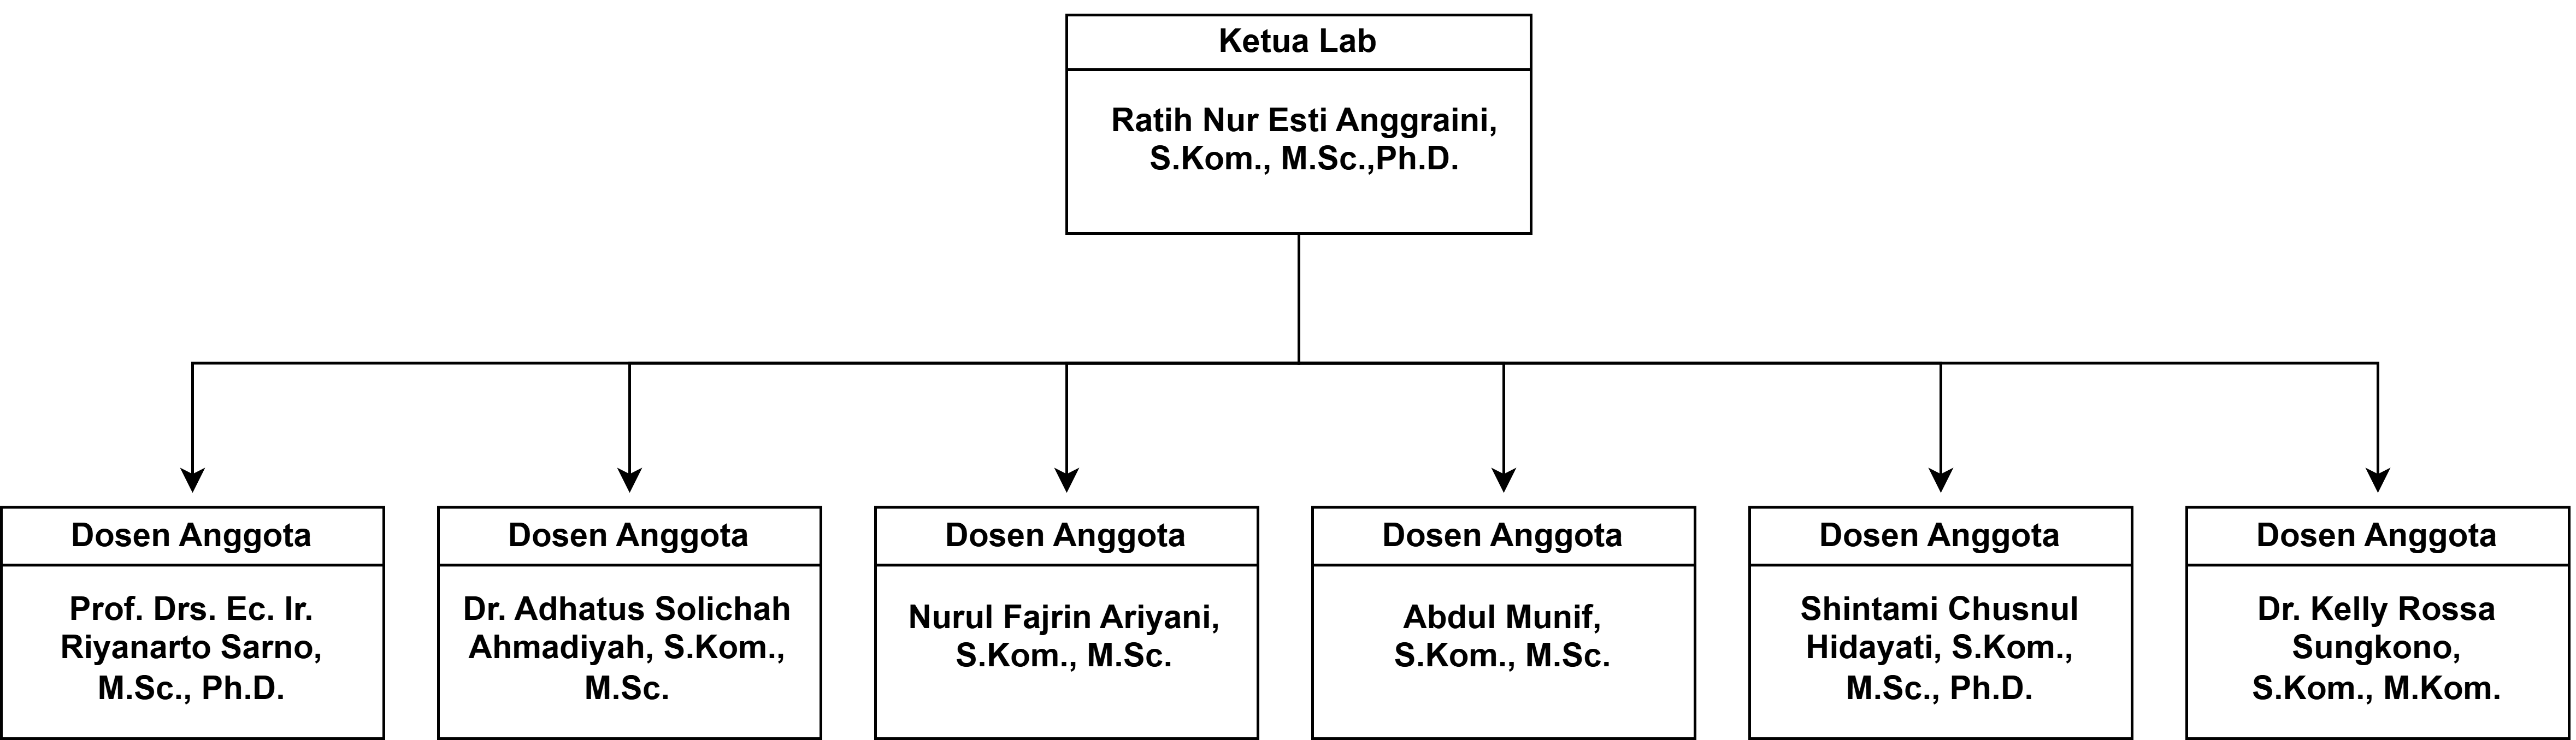
\includegraphics[width=\linewidth]{gambar/struktur-organisasi-mci.png}
	\caption{Struktur Organisasi Laboratorium MCI}
	\label{fig:struktur-organisasi}
\end{figure} 
  \cleardoublepage

  % Bab 3 tunjauan pustaka
  % Ubah kalimat sesuai dengan judul dari bab ini
\chapter{TINJAUAN PUSTAKA}

% Ubah konten-konten berikut sesuai dengan yang ingin diisi pada bab ini

\section{\textit{Magnetic Imaging Resonance}}

\textit{Magnetic Resonance Imaging} (MRI) adalah teknik pencitraan medis non-invasif yang menghasilkan gambar dengan resolusi tinggi dan kontras jaringan lunak yang sangat baik, memungkinkan visualisasi struktur internal tubuh secara detail dalam format tiga dimensi. Dalam lima tahun terakhir, perkembangan signifikan terjadi pada sistem \textit{low-field} MRI yang kini mampu memberikan performa klinis mendekati \textit{high-field} MRI, dengan keunggulan seperti biaya lebih rendah dan keamanan yang lebih baik untuk pasien tertentu \citep{Hori2021,Huo2025}. Selain itu, real-time MRI (RT-MRI) memungkinkan pencitraan proses dinamis secara langsung tanpa perlu pengulangan, sangat berguna untuk organ yang bergerak seperti jantung dan saluran pencernaan, serta dalam panduan prosedur intervensional \citep{Nayak2022}. Dengan kemajuan teknologi ini, MRI menjadi alat diagnostik yang esensial dalam berbagai bidang medis, termasuk neurologi, kardiologi, dan onkologi, dengan kemampuan yang terus ditingkatkan untuk menghasilkan citra berkualitas tinggi dan informasi fungsional yang mendalam \citep{Hori2021,Nayak2022,Thomas2023}

\section{Artefak MRI}

Artefak dalam pencitraan MRI merupakan masalah yang timbul karena akuisisi citra yang lambat dan sekuensial, dimana data dikumpulkan pada k-ruang (\textit{k-space}) \citep{Liu2020}. Dalam pencitraan otak, artefak gerak (\textit{motion artifacts}) adalah jenis degradasi citra yang paling sering ditemui \citep{Sommer2020}. Artefak ini timbul dari gerakan pasien, baik secara sengaja maupun tidak disengaja karena proses yang dibutuhkan untuk mengumpulkan data citra cukup lama \citep{Al-masni2022}. Artefak gerakan biasanya tampak sebagai \textit{blur} atau bayangan (\textit{ghosting}) pada \textit{phase encoding direction}, yang dapat menurunkan kualitas citra hingga tidak dapat digunakan untuk diagnosis \citep{Liu2020}. Bahkan, artefak gerakan dapat memengaruhi 10\% hingga 42\% pemeriksaan MRI otak, dan dapat menimbulkan bias sistematis dalam perkiraan morfometrik struktur otak \citep{Sommer2020, Vakli2023}.

\section{\textit{ResNet}}

ResNet (\textit{Residual Network}) adalah arsitektur \textit{deep neural network} yang dirancang untuk mengatasi masalah degradasi performa pada \textit{deep network} dengan menggunakan mekanisme \textit{residual learning} melalui \textit{shortcut connections} yang melakukan pemetaan identitas dan menambahkan \textit{output}-nya ke \textit{output} pada \textit{stacked layers} \citep{He2015}. Arsitektur ini telah menjadi dasar bagi banyak varian dan pengembangan, seperti Res2Net yang memperkenalkan koneksi residual hierarkis dalam satu blok residual untuk meningkatkan representasi fitur \textit{multiscale}, sehingga meningkatkan kinerja pada berbagai tugas visi komputer \citep{Gao2021}. Dalam bidang pengolahan citra medis, ResNet telah banyak digunakan untuk diagnosis berbagai penyakit seperti tumor paru, kanker payudara, dan gangguan otak, dengan kemampuan adaptasi yang baik terhadap data medis dan memberikan hasil yang baik dalam diagnosis dengan bantuan komputer \citep{Xu2023}.

\section{\textit{DenseNet}}

\section{\textit{EfficientNet}}

\section{\textit{Vision} Transformer (ViT)}

\section{SwinV2 Transformer}

\section{\textit{Generative Adversarial Network}}

\section{Pix2Pix}

\section{Metrik Evaluasi}

\subsection{Metrik Evaluasi Klasifikasi Gambar}

\subsection{\textit{Peak Signal-to-Noise Ratio}}

\subsection{\textit{Structural Similarity Index}}

%% Contoh input gambar dengan format *.jpg
%\begin{figure} [ht] \centering
%  % Nama dari file gambar yang diinputkan
%  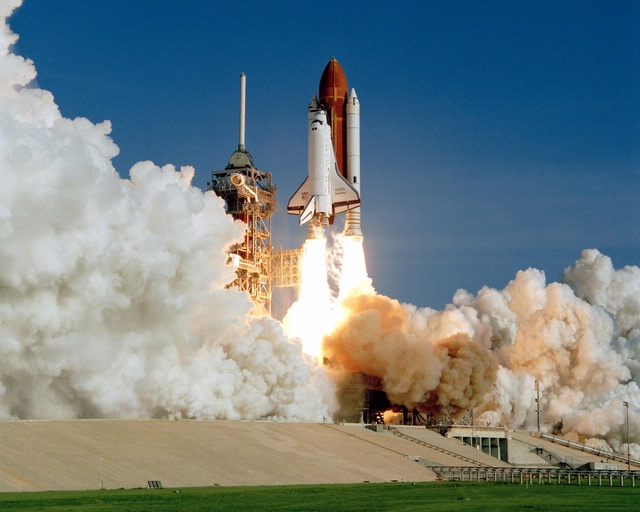
\includegraphics[scale=0.3]{gambar/space-shuttle.jpg}
%  % Keterangan gambar yang diinputkan
%  \caption{Peluncuran pesawat luar angkasa Discovery \citep{DiscoverySpaceShuttle}}
%  % Label referensi dari gambar yang diinputkan
%  \label{fig:SpaceShuttle}
%\end{figure}
%
%Roket luar angkasa merupakan \lipsum[16][1-10]

% Contoh penggunaan referensi dari gambar yang diinputkan
%\emph{Discovery}, Gambar \ref{fig:SpaceShuttle}, merupakan \lipsum[17][1-9]

%\subsection{Hukum Newton}
%
%% Contoh penggunaan referensi dari pustaka
%Newton \citep{Newton1687} pernah merumuskan bahwa \lipsum[19]
%% Contoh penggunaan referensi dari persamaan
%Kemudian menjadi persamaan seperti pada persamaan \ref{eq:FirstNewtonLaw}.
%
%% Contoh pembuatan persamaan
%\begin{equation}
%  % Label referensi dari persamaan yang dibuat
%  \label{eq:FirstNewtonLaw}
%  % Baris kode persamaan yang dibuat
%  \sum \mathbf{F} = 0\; \Leftrightarrow\; \frac{\mathrm{d} \mathbf{v} }{\mathrm{d}t} = 0.
%\end{equation}
%
%\subsection{Anti Gravitasi}
%
%Anti gravitasi merupakan \lipsum[20]

  \cleardoublepage

  % Bab 4 desain dan implementasi
  % Ubah kalimat sesuai dengan judul dari bab ini
\chapter{DESAIN DAN IMPLEMENTASI}

% Ubah konten-konten berikut sesuai dengan yang ingin diisi pada bab ini
\section{Deskripsi Sistem}

Sistem yang dikembangkan dalam kerja praktik ini adalah sebuah kerangka kerja \textit{fault tolerance} untuk pemrosesan citra medis, khususnya MRI otak. Sistem ini dirancang untuk melakukan mitigasi dampak negatif dari artefak gerak (\textit{motion artifacts}) sebelum citra diproses lebih lanjut oleh sistem lanjutan \textit{image captioning}. Secara garis besar, sistem terdiri dari tiga komponen utama yang saling terintegrasi:

\begin{enumerate}[nolistsep]
	\item \textbf{Modul simulasi data} yang bertugas untuk menghasilkan dataset sintetis untuk menyimulasikan artefak gerak yang terjadi di dunia nyata.
	
	\item \textbf{Modul klasifikasi artefak} yang bertugas mendeteksi jenis artefak gerak dengan empat kelas klasifikasi yaitu translasi horizontal, translasi vertikal, rotasi, dan gambar bersih pada citra.
	
	\item \textbf{Modul koreksi citra} yang bertugas merekonstruksi citra dengan artefak menjadi citra bersih.   
\end{enumerate}

\subsection{Desain Pembuatan Dataset Simulasi}

Untuk melatih model koreksi citra dengan Pix2Pix, diperlukan pasangan data citra bersih dan artefak. Sistem ini menggunakan pendekatan simulasi berbasis domain frekuensi (\textit{k-space}) untuk melakukan simulasi artefak gerak sesuai dengan kondisi pada dunia nyata. Proses pembuatan dataset latih ditunjukkan pada Gambar \ref{fig:flowchart-dataset}.

\begin{figure}[H]
	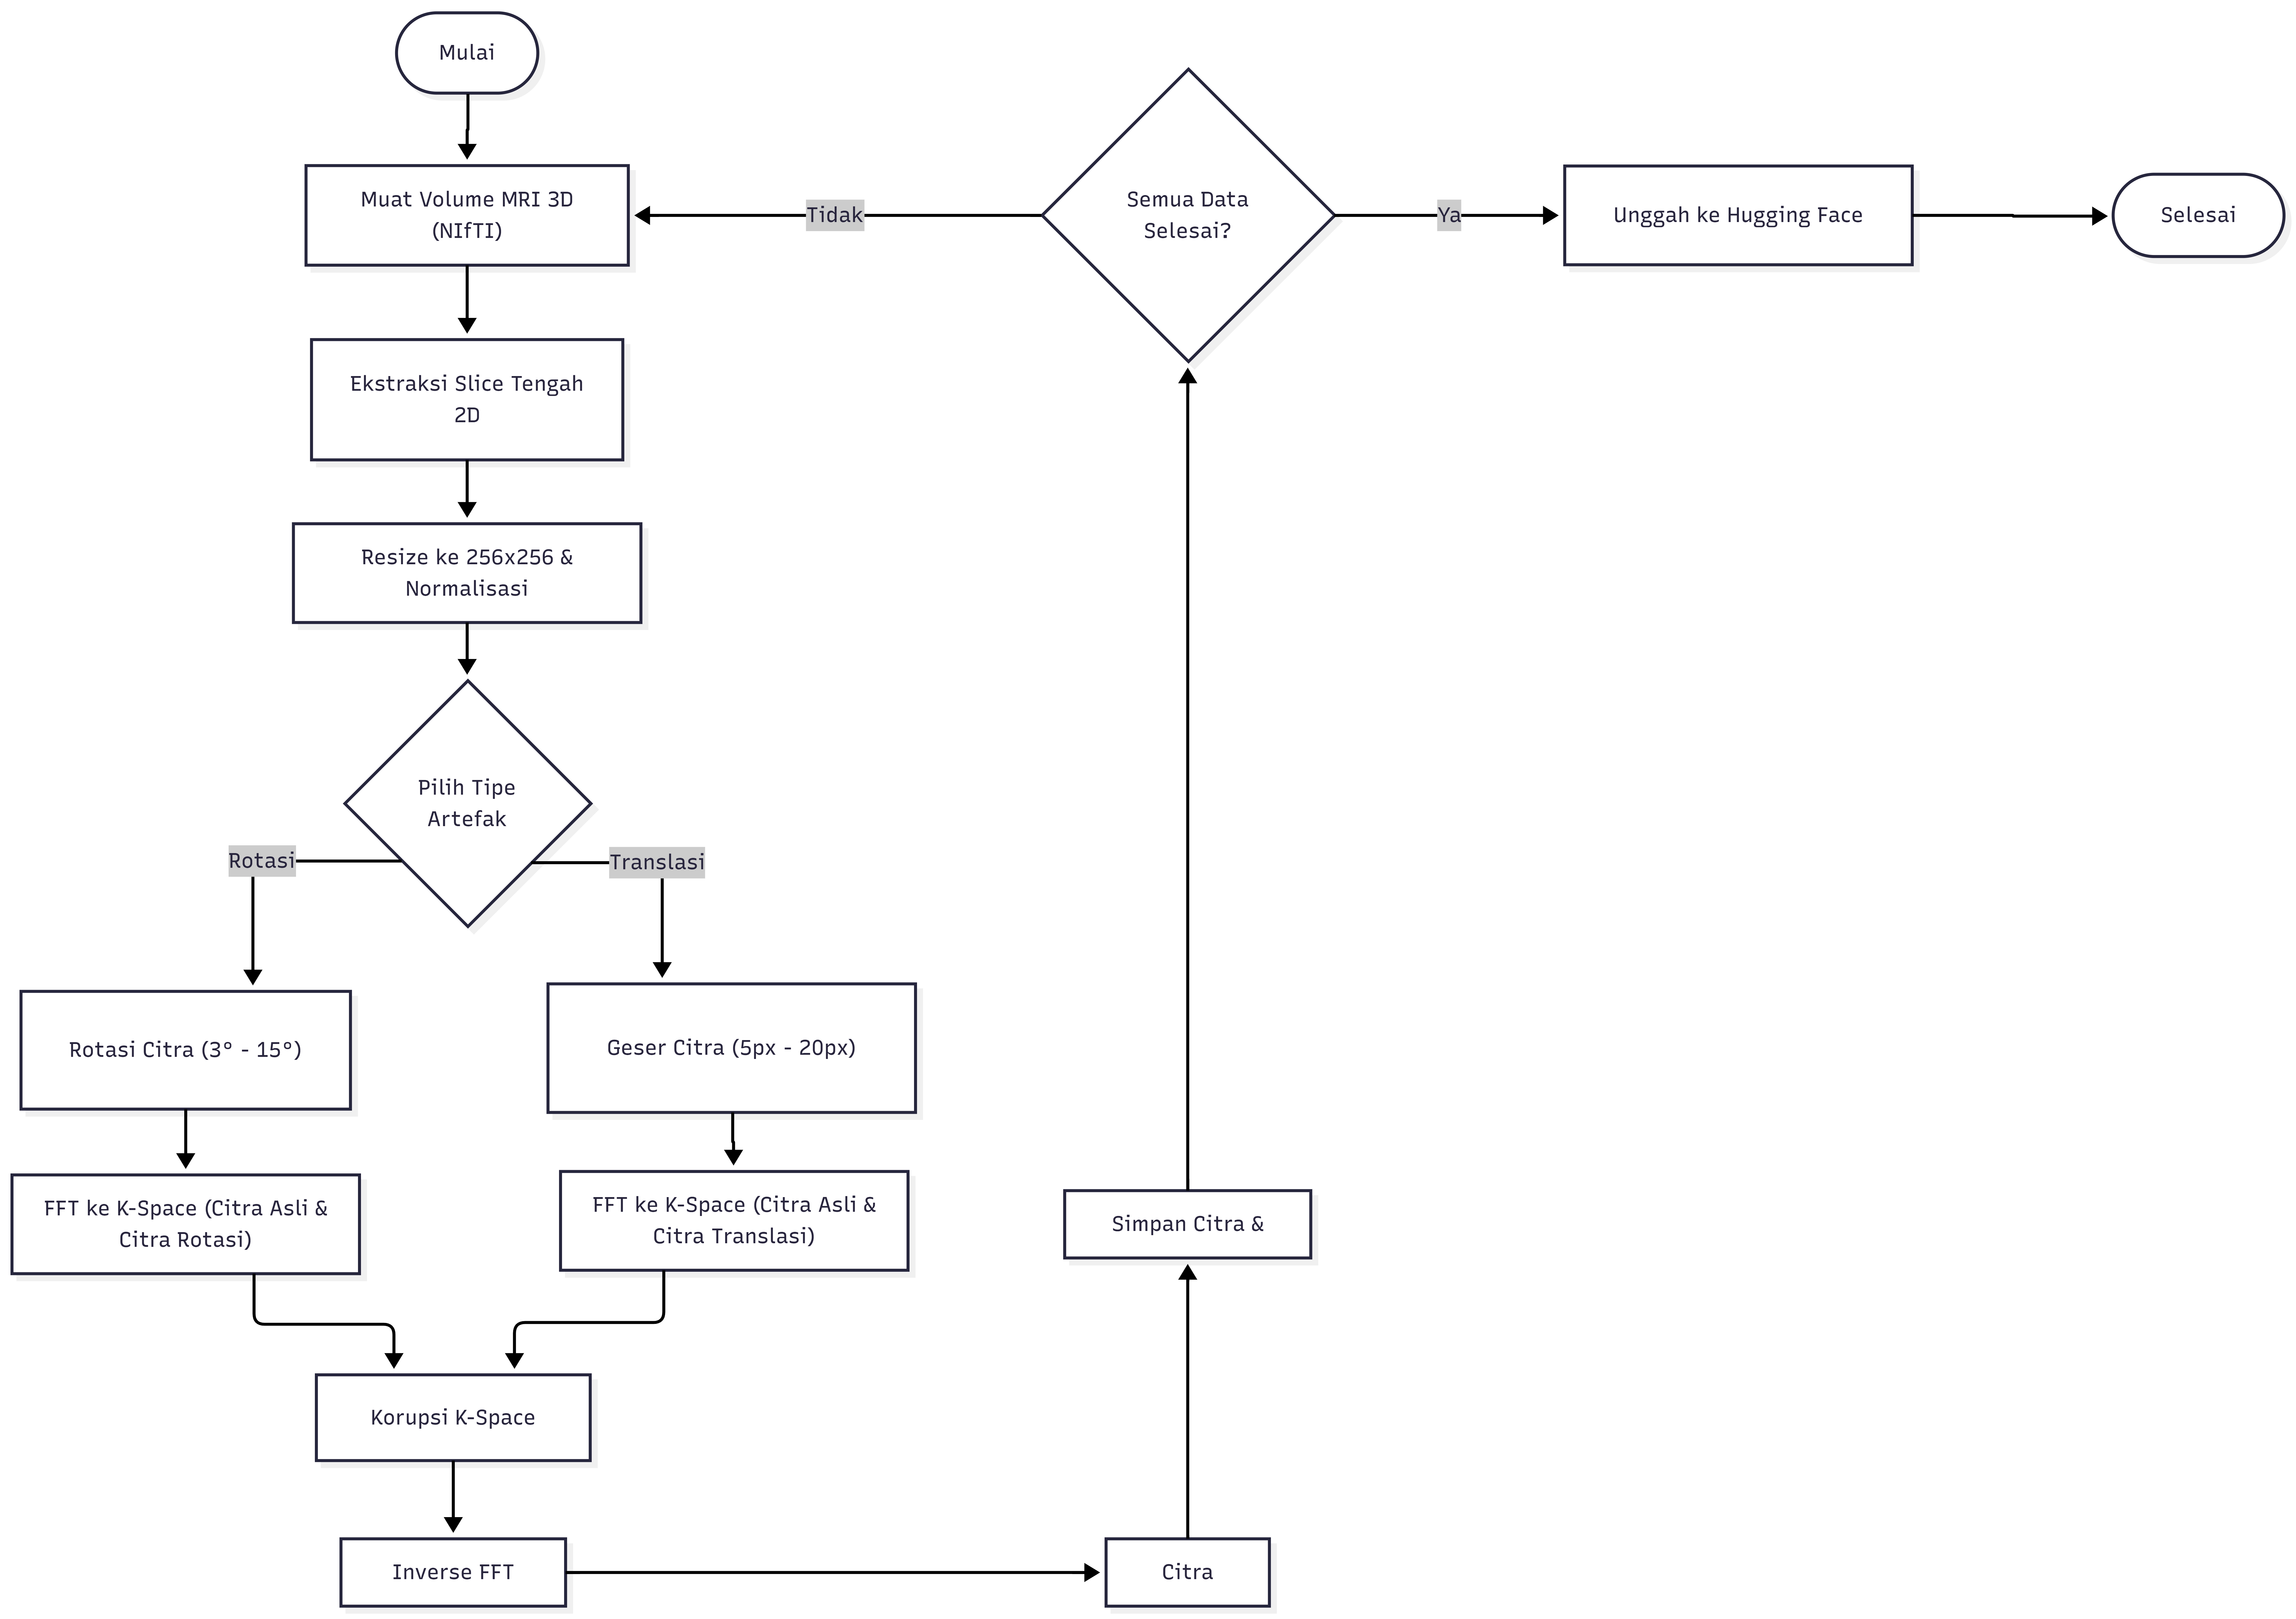
\includegraphics[width=\linewidth]{gambar/flowchart-dataset.png}
	\caption{Diagram Alur Pembuatan Dataset}
	\label{fig:flowchart-dataset}
\end{figure}

Secara umum, proses simulasi artefak terdiri dari tiga bagian, yaitu:

\begin{enumerate}[nolistsep]
	
	\item Transformasi citra bersih ke \textit{k-space} domain frekuensi menggunakan \textit{Fast Fourier Transform} (FFT).
	
	\item Simulasi artefak dengan menggabungkan (\textit{splicing}) garis-garis frekuensi dari citra diam dan citra yang dilakukan translasi atau rotasi. Hal ini meniru inkonsistensi fase yang terjadi ketika pasien bergerak selama pemindaian MRI.
	
	\item Rekonstruksi citra dari data \textit{corrupt k-space} dikembalikan ke domain spasial menggunakan \textit{Inverse FFT} untuk menghasilkan artefak \textit{ghosting} dan \textit{streaking} yang realistis.
	
\end{enumerate}

\subsection{Desain Modul Klasifikasi Artefak}

Modul klasifikasi dirancang menggunakan pendekatan \textit{Transfer Learning} dari model \textit{pre-trained} untuk mengklasifikasikan empat kelas artefak citra, yaitu bersih, \textit{horizontal translation}, \textit{vertical translation}, dan rotasi. Proses klasifikasi secara detail dapat dilihat pada Gambar \ref{fig:flowchart-klasifikasi}.

\begin{figure}[H]
	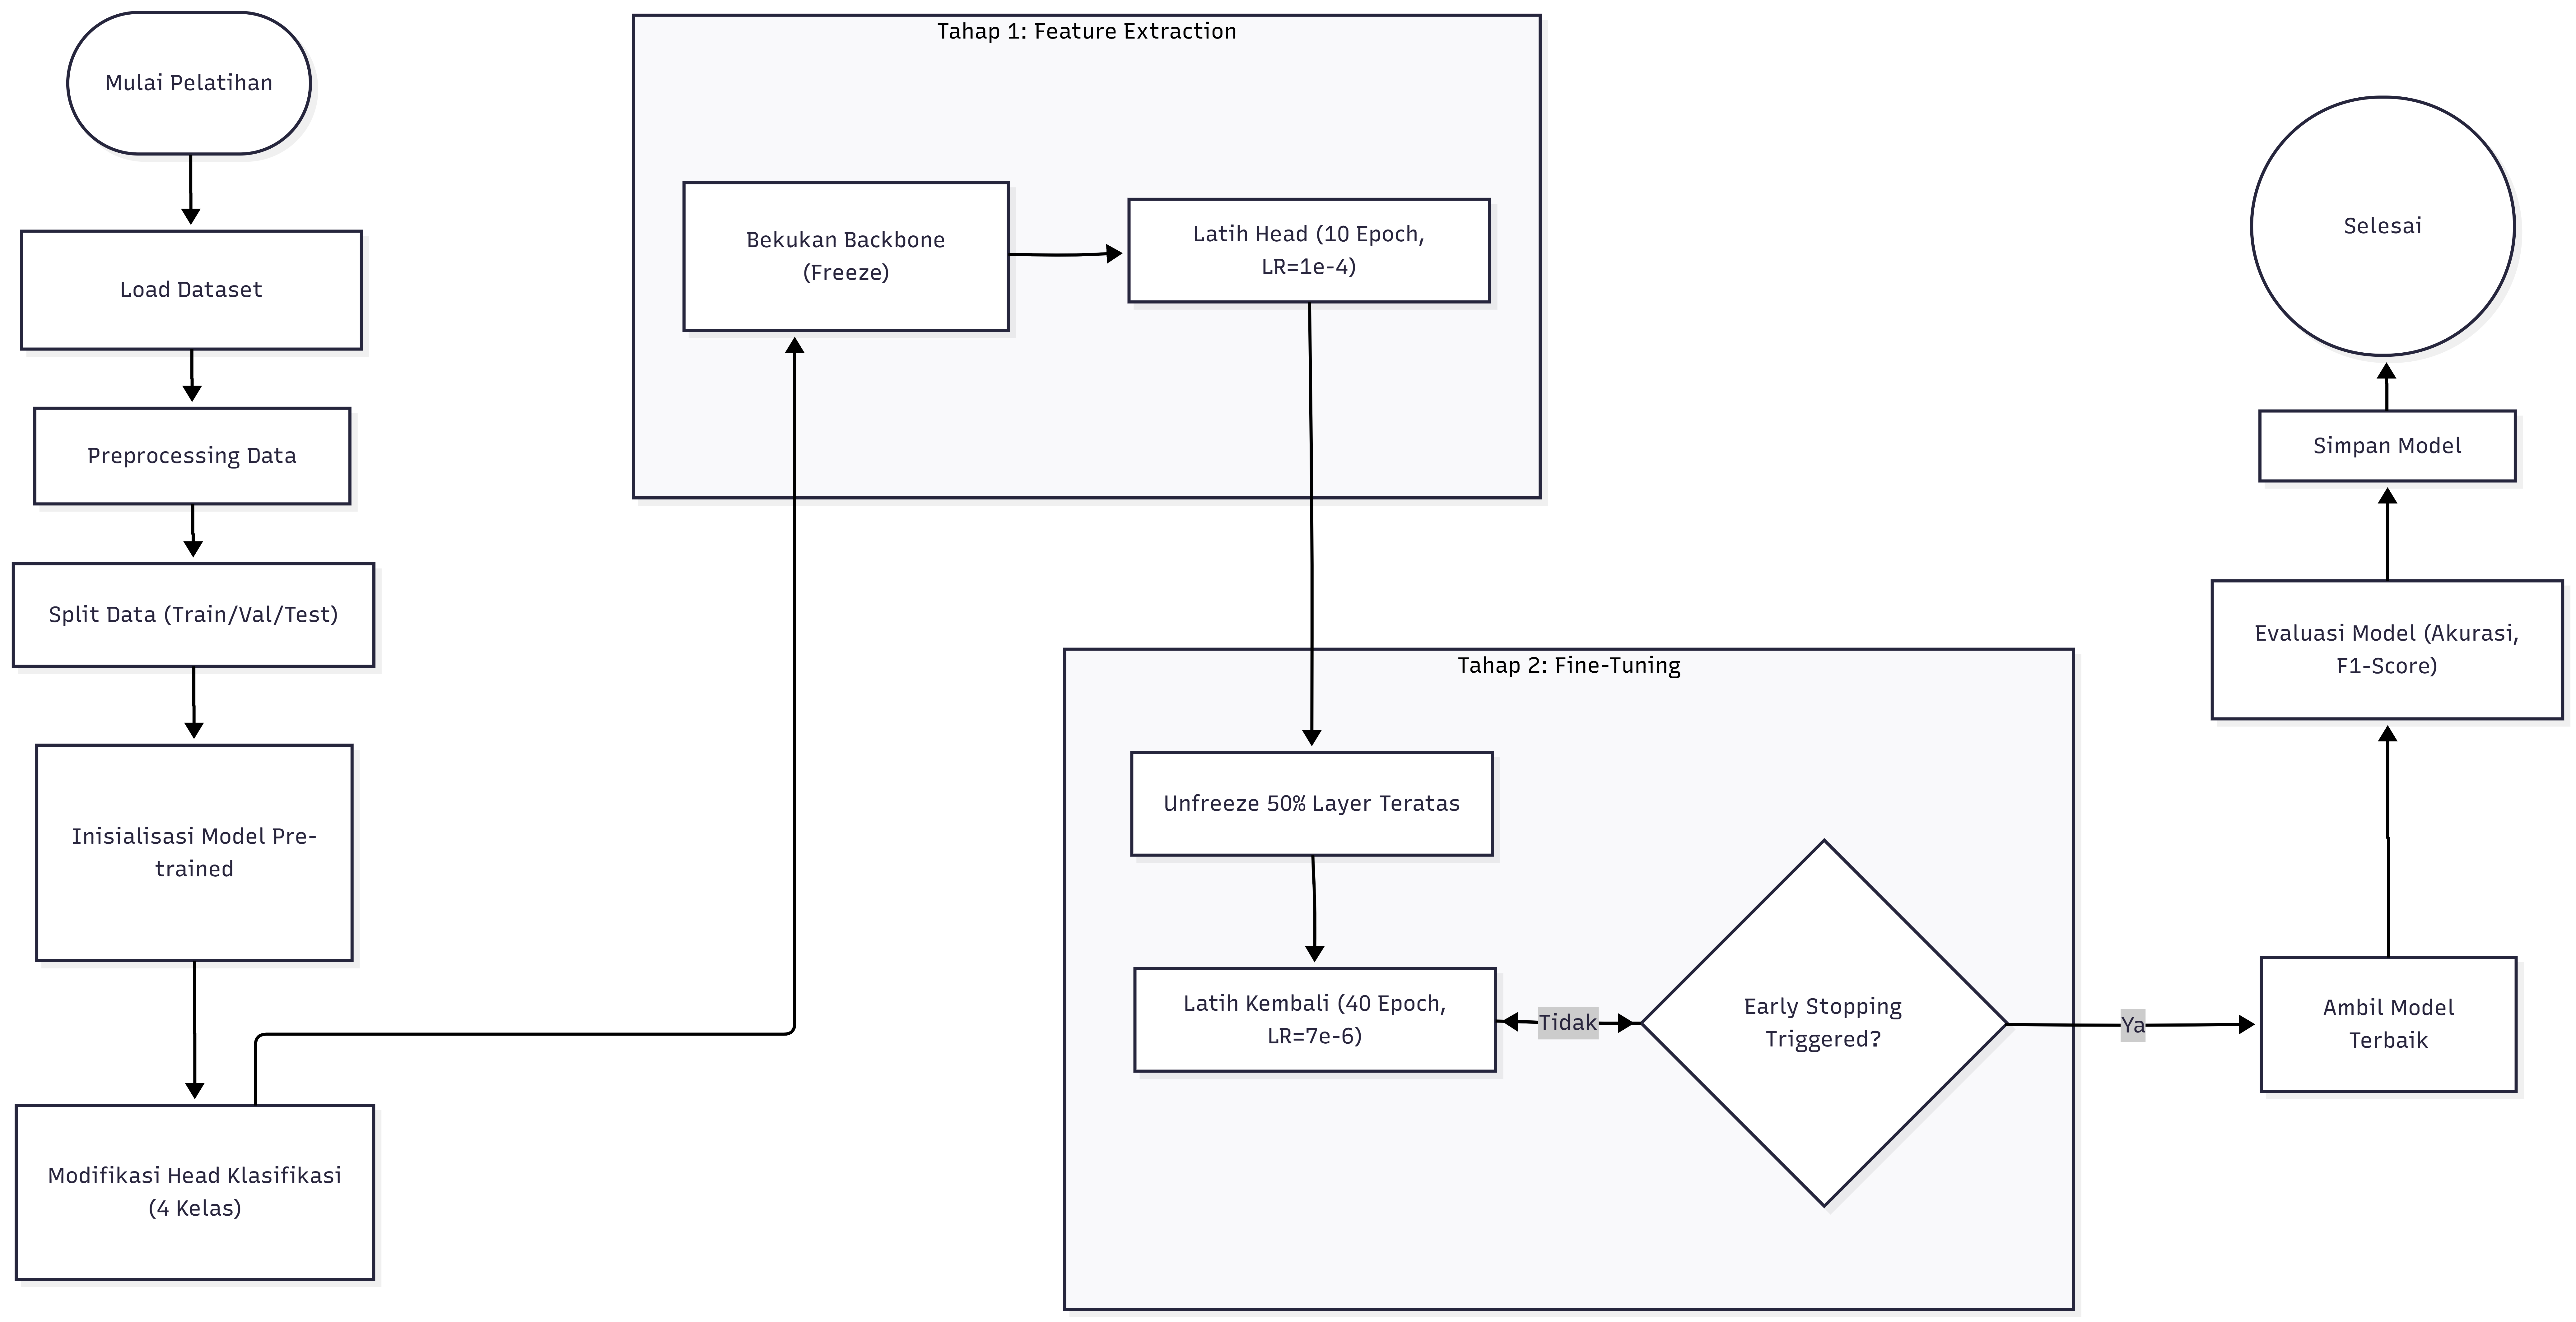
\includegraphics[width=\linewidth]{gambar/flowchart-klasifikasi.png}
	\caption{Diagram Alur Modul Klasifikasi}
	\label{fig:flowchart-klasifikasi}
\end{figure}

Desain modul klasifikasi ini mengeksplorasi dua arsitektur \textit{deep learning} untuk tugas \textit{computer vision}, yaitu \textit{Convolutional Neural Network} (CNN) menggunakan model ResNet, DenseNet, dan EfficientNet serta arsitektur Transformer menggunakan \textit{Vision Transformer} (ViT) dan Swin Transformer. Lapisan akhir setiap model dimodifikasi menjadi \textit{classification head} untuk menghasilkan probabilitas bagi empat kelas target.

\subsection{Desain Modul Koreksi Citra}

Modul koreksi dirancang untuk tugas translasi gambar ke gambar (\textit{image-to-image translation}). Arsitektur yang digunakan adalah Pix2Pix \textit{Conditional GAN} untuk merekonstruksi gambar bersih dari gambar dengan artefak. Arsitektur modul koreksi dapat dilihat pada Gambar \ref{fig:flowchart-koreksi}. 

\begin{figure}[H]
	\centering
	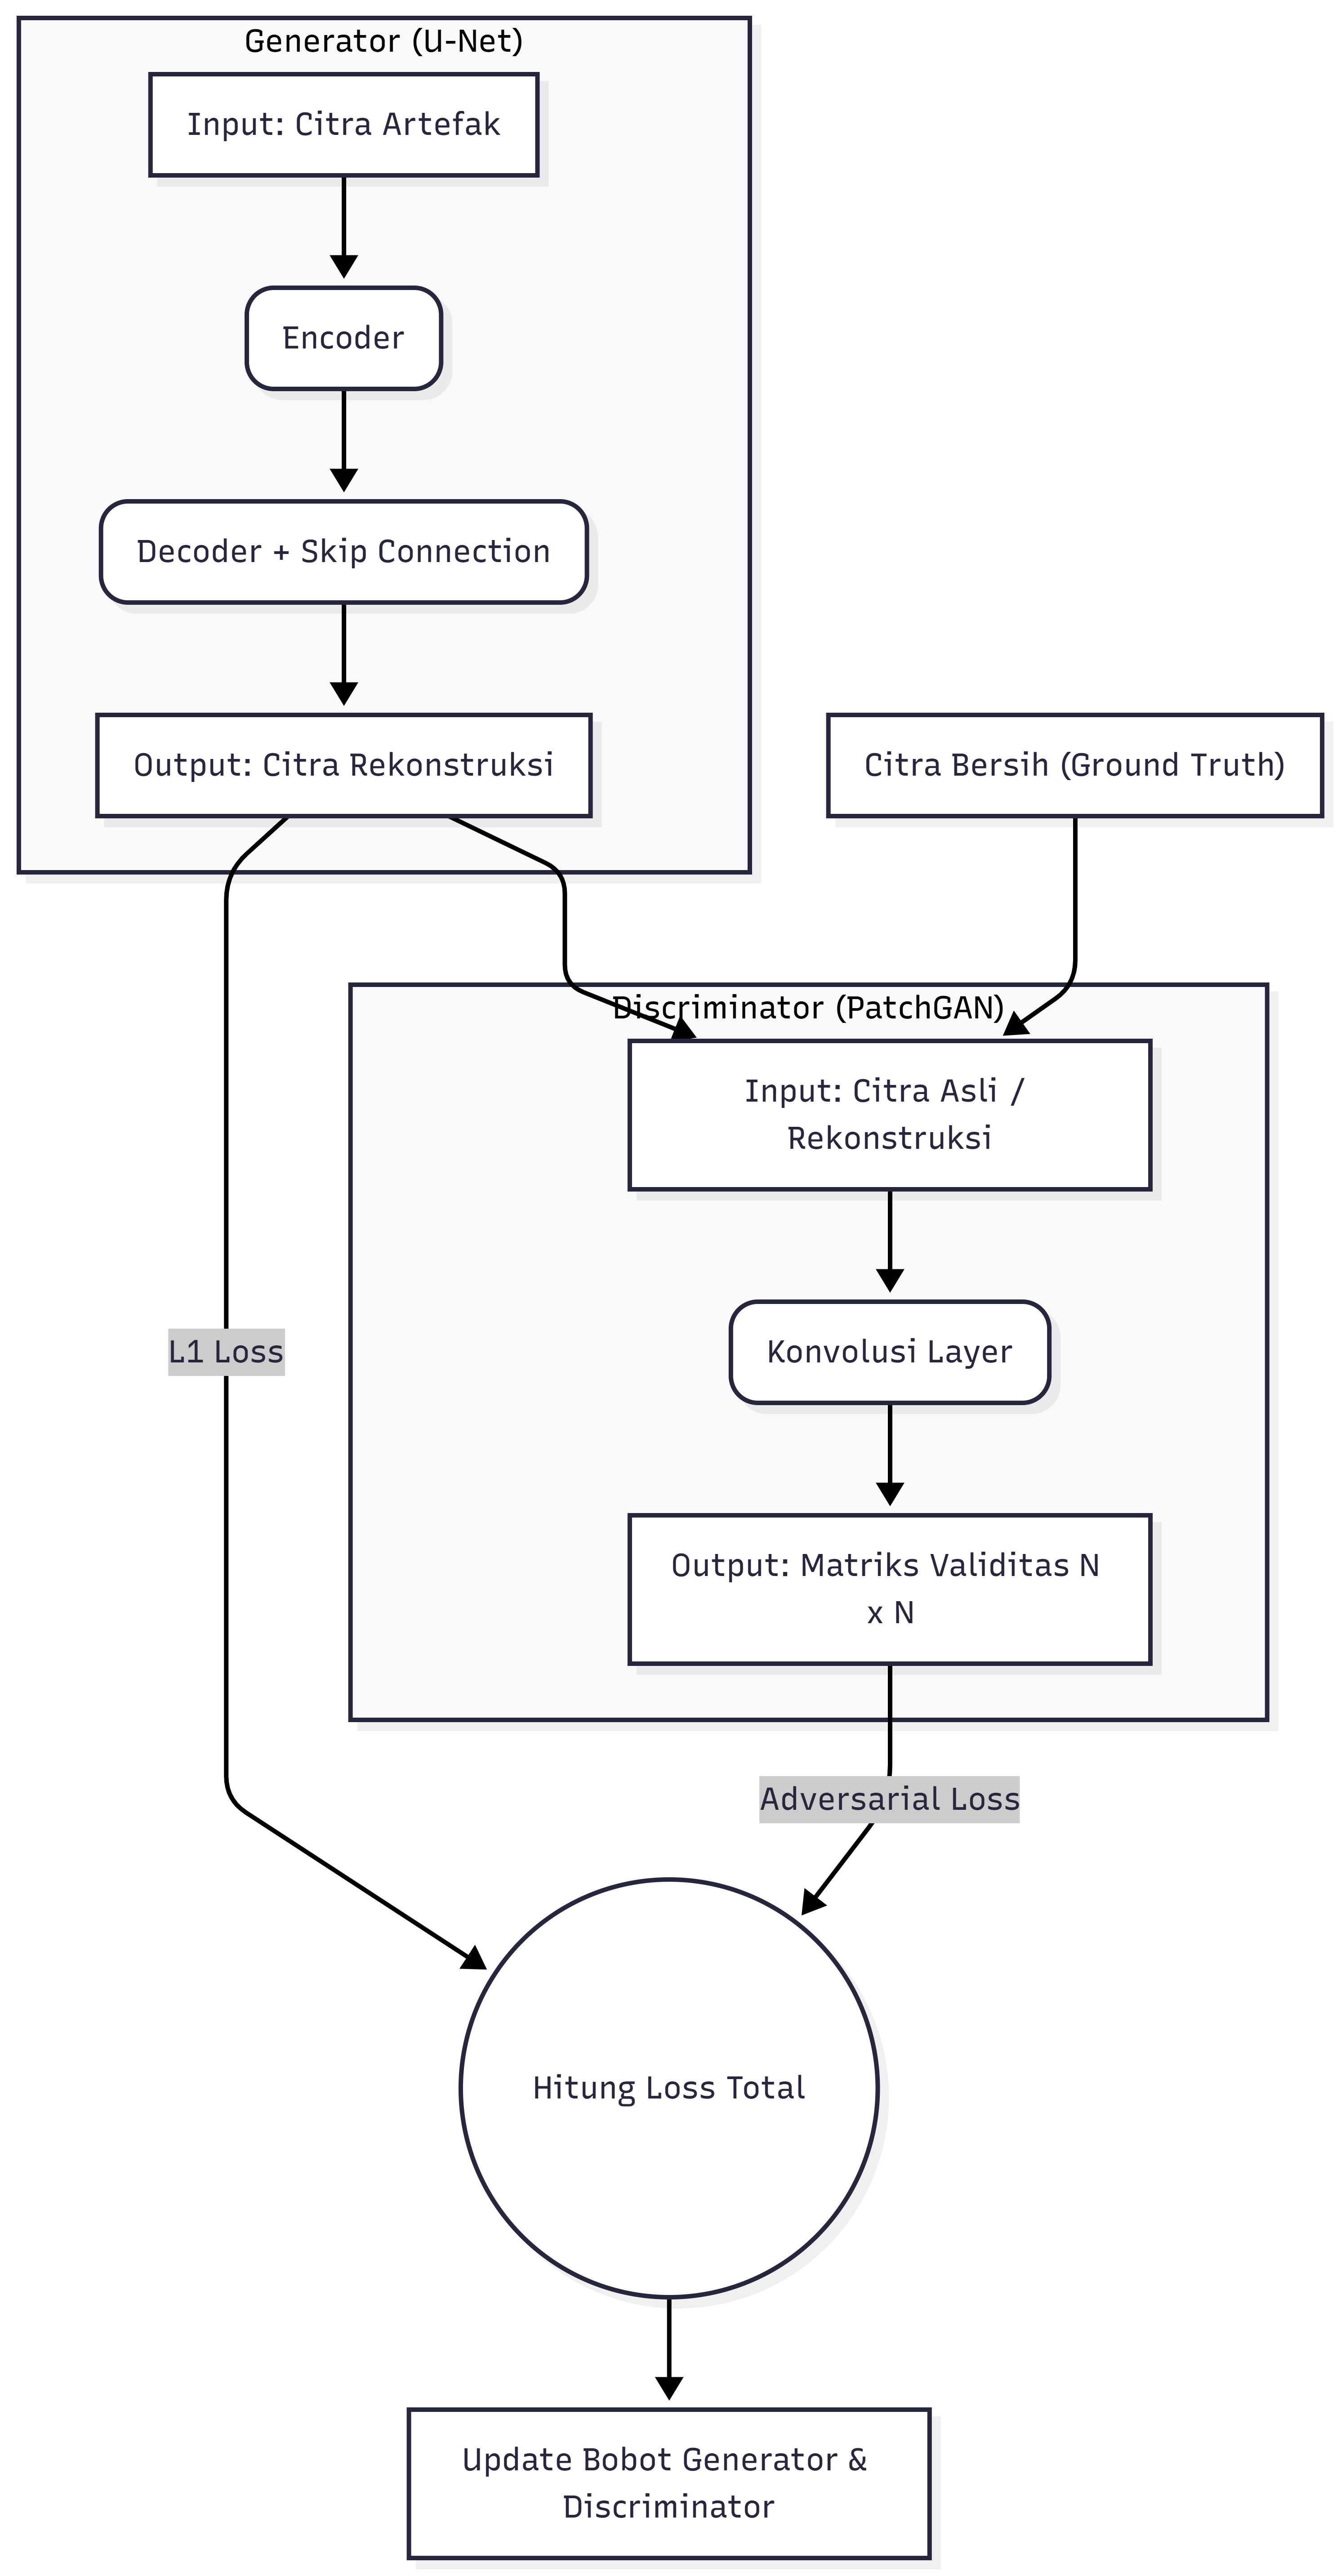
\includegraphics[width=0.5\linewidth]{gambar/flowchart-koreksi.png}
	\caption{Diagram Alur Modul Koreksi Citra}
	\label{fig:flowchart-koreksi}
\end{figure}

Pix2Pix terdiri dari dua komponen yang saling berkompetisi:

\begin{enumerate}[nolistsep]
	\item \textit{Generator} berbasis U-Net yang bertugas menerima input citra dengan artefak dan menghasilkan citra bersih. Arsitektur U-Net digunakan karena adanya \textit{skip connections} yang memungkinkan informasi detail struktur otak dari input tetap terjaga hingga \textit{output}.
	
	\item \textit{Discriminator} berbasis \textit{convolutional PatchGAN} yang bertugas membedakan antara citra bersih asli dan citra hasil rekonstruksi \textit{Generator}. PatchGAN bekerja dengan menilai realisme citra pada level \textit{patch} lokal yang efektif untuk menghasilkan tekstur yang tajam.
\end{enumerate}

\section{Implementasi Sistem}

\subsection{Implementasi Pembuatan Dataset}

\subsection{Implementasi Modul Klasifikasi}

\subsection{Implementasi Modul Koreksi Citra}
Alat diimplementasikan dengan \lipsum[22]

% Contoh pembuatan code snippet
\begin{lstlisting}[
  language=C++,
  label={lst:Hello World},
  caption={Program hello world}
]
#include <iostream>

int main() {
    std::cout << "Hello World!";
    return 0;
}
\end{lstlisting}

% Contoh penggunaan referensi dari code snippet yang diinputkan
Seperti contoh pada baris program Listing \ref{lst:Hello World} dan Listing \ref{lst:PrimeNumber}, \lipsum[23]

% Contoh input code snippet
\lstinputlisting[
  % Bahasa yang digunakan oleh code snippet
  language=Python,
  % Label referensi dari code snippet yang diinputkan
  label={lst:PrimeNumber},
  % Keterangan dari code snippet yang diinputkan
  caption={Program perhitungan bilangan prima}
% Nama dari file code snippet yang diinputkan
]{program/prime-number.py}

  \cleardoublepage

  % Bab 5 pengujian dan evaluasi
  % Ubah kalimat sesuai dengan judul dari bab ini
\chapter{PENGUJIAN DAN EVALUASI}

Bab ini membahas skenario pengujian yang dilakukan untuk memvalidasi kinerja sistem serta hasil evaluasi dari modul klasifikasi dan modul koreksi. Pengujian bertujuan untuk memastikan bahwa model yang dibangun mampu mengenali jenis artefak dengan akurat dan memperbaiki citra yang rusak secara efektif.

\section{Skenario Pengujian}

Skenario pengujian dirancang untuk mengukur kinerja model dalam lingkungan yang terkontrol namun representatif terhadap masalah yang dihadapi. Pengujian dilakukan secara terpisah untuk modul klasifikasi dan modul koreksi.

\subsection{Lingkungan Pengujian}

Seluruh proses pelatihan dan pengujian dilakukan menggunakan platform Kaggle Notebook. Lingkungan ini menyediakan spesifikasi perangkat keras berupa satu GPU NVIDIA Tesla P100 dan RAM sebesar 32 GB yang memadai untuk komputasi \textit{deep learning}. Perangkat lunak utama yang digunakan adalah bahasa pemrograman Python 3.10 dengan dukungan \textit{library} Tensorflow, Pytorch, Transformers, Pandas, NumPy, dan Matplotlib. 

\subsection{Skenario Pengujian Modul Klasifikasi}

Pengujian modul klasifikasi bertujuan membandingkan performa antara arsitektur CNN dan Transformer. Dalam pelaksanaannya, dataset dibagi menjadi data latih (\textit{training set}) yang digunakan untuk melatih bobot model dan data uji (\textit{test set}) yang digunakan sebagai data validasi untuk memantau metrik performa seperti \textit{validation loss} dan akurasi pada setiap epoch. Data uji juga digunakan sebagai acuan dalam penerapan mekanisme \textit{early stopping} untuk mencegah terjadinya \textit{overfitting}.

Konfigurasi \textit{hyperparameter} ditetapkan secara seragam pada aspek-aspek umum untuk memastikan perbandingan yang adil antara model CNN (ResNet50, DenseNet121, EfficientNetB0) dan Transformer (ViT, Swin Transformer). Meskipun demikian, penyesuaian khusus tetap dilakukan pada komponen \textit{optimizer} dan regularisasi agar kinerja masing-masing arsitektur dapat mencapai titik optimal. Rincian lengkap mengenai konfigurasi tersebut disajikan pada Tabel \ref{tb:hyperparameter}

%Inout tabel hyperaparameter
% Contoh pembuatan tabel
\begin{longtable}{|p{2cm}|p{4cm}|p{4cm}|}
  % Keterangan dari tabel yang dibuat
  \caption{Konfigurasi \textit{Hyperparameter} Model Klasifikasi}
  % Label referensi dari tabel yang dibuat
  \label{tb:hyperparameter}\\
  % Isi dari tabel yang dibuat
  \hline
  \rowcolor[HTML]{C0C0C0}
  \textbf{Parameter} & \textbf{Konfigurasi CNN} & \textbf{Konfigurasi Transformer} \\ \hline
  \textit{Input Size} & ResNet \& DenseNet: $256 \times 256$, EfficientNet: $224 \times 224$ & SwinV2: $224 \times 224$, ViT: $256 \times 256$ \\ \hline
  \textit{Batch Size} & 32 & 32 \\ \hline
  \textit{Optimizer} & Adam & AdamW \\ \hline
  \textit{Learning Rate} & \textit{Warm Up}:$1e-4$, \textit{Fine tune}: $7e-6$ & $1e-4$ \\ \hline
  Epochs & \textit{Warm Up}: 10, \textit{Fine Tune}: 40 & 20 \\ \hline
  Regularisasi & \textit{Dropout (0.5)}, \textit{Early Stopping (Patience=5)}& \textit{Weight Decay (0.01), Early Stopping (Patience=5)} \\ \hline
  Augmentasi & \textit{RandomFlip, RandomZoom} & \textit{RandomFlip, ColorJitter, RandomResizedCrop} \\ \hline
\end{longtable}
 

Setelah proses pelatihan selesai, kinerja model dievaluasi secara menggunakan empat metrik klasifikasi utama. Akurasi (\textit{Accuracy}) digunakan untuk melihat rasio prediksi yang benar terhadap keseluruhan data. Presisi (\textit{Precision}) dihitung untuk mengukur ketepatan prediksi positif model terhadap data aktual, yang sangat penting untuk meminimalkan \textit{false positive}. \textit{Recall} (sensitivitas) digunakan untuk mengukur kemampuan model dalam menemukan kembali seluruh informasi yang relevan. Terakhir, F1-Score digunakan sebagai rata-rata harmonik antara presisi dan \textit{recall} untuk memberikan gambaran kinerja yang seimbang pada dataset \textit{multi-class}.

\subsection{Skenario Pengujian Modul Koreksi}

Pengujian modul koreksi difokuskan untuk menilai kemampuan \textit{Generator} dalam arsitektur Pix2Pix GAN untuk merekonstruksi citra bersih dari citra dengan artefak. Model dilatih dengan input citra berukuran $256 \times 256$ piksel selama 250 epoch. Proses optimasi menggunakan algoritma Adam dengan parameter momentum $\beta_1=0.5$ dan $\beta_2=0.999$, serta learning rate konstan sebesar $2e-4$. Dalam fungsi \textit{loss} gabungan, bobot $\lambda$ diatur sebesar 100. Nilai ini dipilih untuk memberikan prioritas yang jauh lebih tinggi pada L1 \textit{Loss} (kemiripan piksel absolut) dibandingkan \textit{Adversarial Loss}. Tujuannya adalah memastikan struktur anatomi otak tetap terjaga dan tidak berubah bentuk meskipun teksturnya diperbaiki oleh GAN.

Kualitas citra hasil rekonstruksi kemudian dievaluasi menggunakan dua metrik standar dalam pemrosesan citra medis. Metrik pertama adalah \textit{Peak Signal-to-Noise Ratio} (PSNR) yang mengukur rasio antara nilai maksimum sinyal dan noise dalam satuan desibel (dB); nilai yang lebih tinggi mengindikasikan kualitas rekonstruksi yang lebih baik. Metrik kedua adalah \textit{Structural Similarity Index} (SSIM) yang mengukur kemiripan struktural (luminansi, kontras, dan struktur) antara citra hasil koreksi dengan citra asli (\textit{ground truth}). Nilai SSIM berkisar antara -1 hingga 1. Nilai yang mendekati 1 menunjukkan bahwa struktur citra hasil rekonstruksi sangat identik dengan aslinya.

\section{Evaluasi Pengujian}

Bagian ini memaparkan hasil eksperimen berdasarkan skenario yang telah ditetapkan di atas, mencakup analisis kuantitatif dan kualitatif.

\subsection{Evaluasi Modul Klasifikasi Artefak}

Berdasarkan pelatihan yang dilakukan pada lima model berbeda, diperoleh hasil evaluasi kuantitatif pada data uji. Rangkuman mengenai metrik terbaik yang dicapai oleh masing-masing model ditunjukkan pada Tabel \ref{tb:classificationperf}.

% Gunakan environment 'table' dengan opsi [H] agar tabel tidak terpotong
\begin{table}[H]
	\centering
	\caption{Perbandingan Kinerja Metrik Model Klasifikasi}
	\label{tb:classificationperf}
	
	\vspace{2ex}
	
	% Gunakan tabularx agar lebar pas \textwidth
	% X = Kolom fleksibel (rata kiri, auto wrap)
	% c = Kolom tengah (centered) untuk angka
	\begin{tabularx}{\textwidth}{|X|c|c|c|c|}
		\hline
		\rowcolor[HTML]{C0C0C0}
		\textbf{Model} & \textbf{Akurasi} & \textbf{Presisi} & \textbf{\textit{Recall}} & \textbf{\textit{F1-Score}} \\ \hline
		
		\textbf{ResNet50} & 0.8890 & 0.9053 & 0.8890 & 0.8908 \\ \hline
		\textbf{DenseNet121} & 0.9031 & 0.9106 & 0.9031 & 0.9035 \\ \hline
		\textbf{EfficientNetB0} & 0.8469 & 0.8586 & 0.8469 & 0.8490 \\ \hline
		\textbf{ViT} & 0.8876 & 0.8923 & 0.8876 & 0.8881 \\ \hline
		\textbf{SwinV2 Transformer} & 0.9382 & 0.9539 & 0.9537 & 0.9536 \\ \hline
		
	\end{tabularx}
\end{table}

Analisis hasil menunjukkan bahwa model SwinV2 Transformer mencapai kinerja tertinggi secara konsisten di semua metrik dengan akurasi 93.82\% dan F1-Score 95.36\%. Keunggulan yang signifikan ini disebabkan oleh mekanisme \textit{shifted window attention} yang efektif menangkap konteks lokal maupun global pada citra artefak.

Pada model berbasis CNN, DenseNet menunjukkan kinerja yang paling tinggi dengan akurasi 90.31\% mengungguli ResNet (88.90\%). Hal ini menunjukkan bahwa \textit{dense connections} pada DenseNet membantu dalam propagasi fitur yang lebih efisien dibandingkan \textit{residual connections} pada ResNet untuk tugas klasifikasi ini. Namun, secara keseluruhan, arsitektur Transformer menunjukkan potensi yang lebih besar dengan SwinV2 Transformer secara signifikan mengungguli model-model lainnya.

\begin{figure}[H]
	\centering
	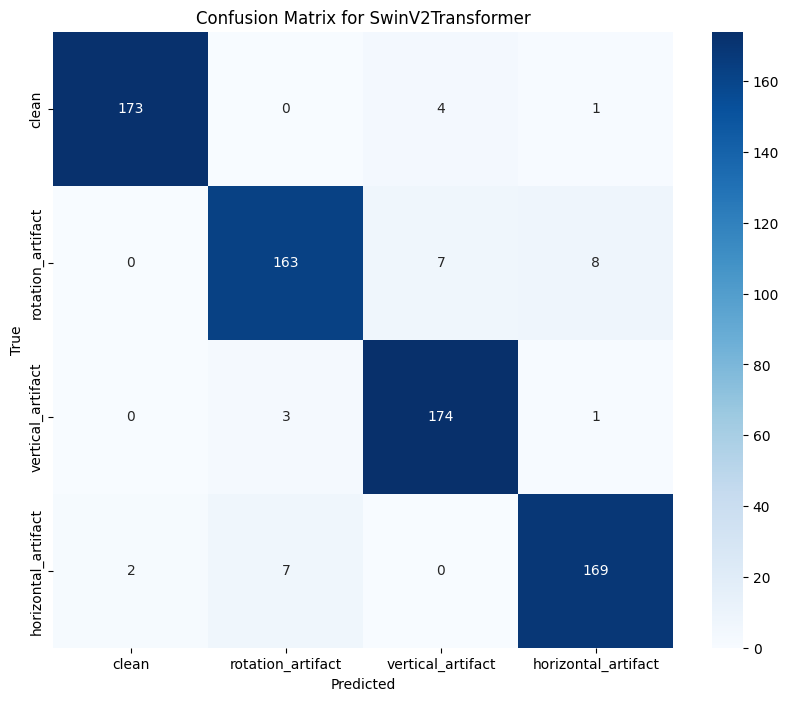
\includegraphics[width=0.9\linewidth]{gambar/swinv2-confusionmatrix.png}
	\caption{\textit{Confusion Matrix} Model Terbaik (SwinV2 Transformer)}
	\label{fig:confusionmatrixswinv2}
\end{figure}


Analisis lebih mendalam dilakukan menggunakan \textit{Confusion Matrix} pada model terbaik (SwinV2 Transformer) yang ditunjukkan pada Gambar \ref{fig:confusionmatrixswinv2} untuk memahami karakteristik prediksi model secara spesifik pada tiap kelas.

\begin{sloppypar}
	Analisis lebih mendalam terhadap Confusion Matrix pada model SwinV2 Transformer menunjukkan karakteristik prediksi yang sangat kuat dalam membedakan citra bersih dari citra dengan artefak. Namun, terdapat pola misklasifikasi yang spesifik jika ditinjau antar kategori artefak. Kesalahan prediksi paling signifikan terjadi pada diferensiasi antara artefak horizontal dengan artefak rotasi, dilanjutkan oleh kesalahan dalam membedakan artefak vertikal dengan artefak rotasi. Selain itu, terdapat pula kecenderungan model salah mengklasifikasikan artefak rotasi sebagai artefak horizontal, dengan frekuensi tertinggi mencapai 8 sampel pada kategori tersebut. Fenomena ini mengindikasikan bahwa pada irisan otak tertentu, distorsi spasial yang dihasilkan oleh gerakan rotasi memiliki kemiripan fitur tekstur dengan pola \textit{ghosting} atau \textit{blurring} linear yang dihasilkan oleh gerakan translasi secara horizontal maupun vertikal. Hal ini menyebabkan batas keputusan model menjadi sedikit samar di antara jenis-jenis gerakan tersebut.
\end{sloppypar}

\subsection{Evaluasi Modul Koreksi Citra}

Pengujian modul koreksi dilakukan dengan membandingkan citra berartefak dan citra hasil restorasi \textit{Generator} terhadap citra asli untuk melihat seberapa baik kemiripan citra yang  dikoreksi dengan citra aslinya jika dibandingkan dengan citra berartefak. Hasil evaluasi dari 200 sampel gambar tes ditunjukkan pada Tabel \ref{tb:gan-perf}. 

% Gunakan environment 'table' dengan opsi [H] agar tabel tidak terpotong
\begin{table}[H]
	\centering
	\caption{Perbandingan Kinerja Metrik Model Klasifikasi}
	\label{tb:gan-perf}
	
	\vspace{2ex}
	
	% Gunakan tabularx agar lebar pas \textwidth
	% X = Kolom fleksibel (rata kiri, auto wrap)
	% c = Kolom tengah (centered) untuk angka
	\begin{tabularx}{\textwidth}{|X|c|c|c|}
		\hline
		\rowcolor[HTML]{C0C0C0}
		\textbf{Metrik} & \textbf{Gambar Berartefak} & \textbf{Gambar Koreksi} & \textbf{Perbedaan}\\ \hline
		
		\textbf{PSNR} & 34.3287 dB & 32.8180 dB & -1.5107  \\ \hline
		\textbf{SSIM} & 0.9061 & 0.9099 & +0.0038 \\ \hline
	\end{tabularx}
\end{table}

Berdasarkan tabel evaluasi kuantitatif, hasil pengujian menunjukkan peningkatan nilai SSIM pada gambar hasil koreksi dibandingkan dengan baseline gambar berartefak. Peningkatan ini mengindikasikan bahwa model GAN berhasil merestorasi integritas struktural dan geometri anatomis citra medis, sehingga \textit{motion artifact} yang mengganggu visualisasi berhasil direduksi. Sebaliknya, nilai PSNR mengalami penurunan setelah dilakukan koreksi. Penurunan ini menunjukkan bahwa meskipun kualitas visual membaik, terdapat deviasi pada intensitas piksel absolut yang kemungkinan disebabkan oleh \textit{micro-texture generation} atau pergeseran piksel minor yang dilakukan oleh generator untuk meningkatkan ketajaman gambar. Hasil ini menegaskan bahwa model lebih berfokus pada kualitas kemiripan struktur gambar dibandingkan dengan kualitas akurasi pada level piksel.


\begin{figure}[H]
	\centering
	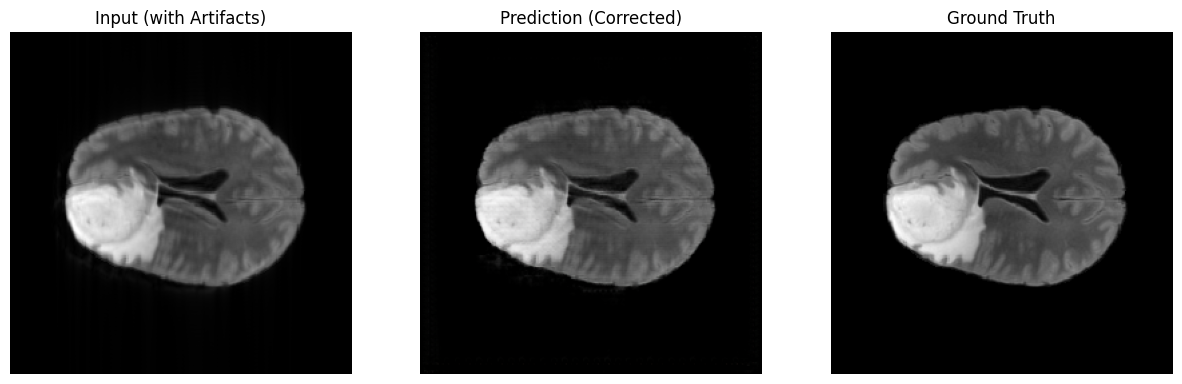
\includegraphics[width=\linewidth]{gambar/gan-image-correction.png}
	\caption{Perbandingan Visual Hasil Koreksi Citra MRI}
	\label{fig:ganimagecompare}
\end{figure}

Secara kualitatif, Gambar \ref{fig:ganimagecompare} menunjukkan kemampuan model dalam meningkatkan ketajaman visual citra yang semula kabur akibat artefak \textit{ghosting}. Alih-alih sekadar mencocokkan intensitas piksel, \textit{Generator} berfokus pada rekonstruksi tekstur dan tepi organ agar terlihat realistis. Hasilnya adalah area latar belakang menjadi lebih bersih dan garis-garis anatomis otak terlihat jauh lebih terlihat dibandingkan citra input. Peningkatan kualitas visual ini mengindikasikan bahwa model memprioritaskan pemulihan fitur-fitur penting yang diperlukan untuk interpretasi visual, meskipun secara statistik terdapat penurunan intensitas sinyal absolut.

  \cleardoublepage

  % Bab 6 kesimpulan dan saran
  \chapter{KESIMPULAN DAN SARAN}

% Ubah konten-konten berikut sesuai dengan yang ingin diisi pada bab ini

\section{Kesimpulan}

Berdasarkan seluruh rangkaian kegiatan kerja praktik yang telah dilakukan mulai dari perancangan hingga pengujian sistem \textit{fault tolerance} untuk mitigasi artefak gerak pada citra MRI otak, dapat ditarik beberapa kesimpulan utama sebagai berikut.

\begin{enumerate}[nolistsep]

  \item Simulasi artefak gerak berupa translasi dan rotasi berhasil dilakukan dengan memanipulasi data citra pada domain frekuensi (\textit{k-space}) untuk menghasilkan dataset pelatihan sintetis yang realistis dan meniru inkonsistensi pada mesin MRI.

  \item Pengembangan model klasifikasi menggunakan strategi transfer learning menunjukkan bahwa arsitektur berbasis Transformer, terutama SwinV2 Transformer, memiliki keunggulan dibandingkan arsitektur CNN dalam menangkap pola artefak yang kompleks baik secara lokal maupun global.

  \item Modul koreksi artefak berhasil dikembangkan menggunakan arsitektur Pix2Pix GAN yang mampu memulihkan detail anatomi sekaligus menghilangkan pola \textit{ghosting} dan \textit{blurring} pada citra dengan memanfaatkan fungsi \textit{loss} gabungan.
  
  \item Hasil evaluasi menunjukkan kinerja sistem yang sangat baik dimana modul klasifikasi terbaik mencapai akurasi 93,82\% dan hasil generasi gambar modul koreksi menghasilkan kenaikan skor SSIM dibandingkan dengan gambar dengan artefak meskipun skor PSNR menunjukkan penurunan, yang menunjukkan bahwa model berfokus pada pemulihan fitur-fitur penting yang meningkatkan kualitas visual gambar dibandingkan dengan perbaikan kualitas pada level piksel.

\end{enumerate}

\section{Saran}

Untuk meningkatkan kinerja dan memperluas cakupan sistem ini di masa mendatang, terdapat beberapa langkah strategis yang dapat dikembangkan lebih lanjut.

\begin{enumerate}[nolistsep]

  \item Pengembangan selanjutnya disarankan dapat mencakup jenis artefak medis lainnya yang sering ditemui dalam MRI seperti artefak \textit{aliasing} atau \textit{noise} frekuensi tinggi agar sistem memiliki cakupan proteksi yang lebih menyeluruh.

  \item Transisi dari pemrosesan irisan dua dimensi menuju pemrosesan volume MRI tiga dimensi secara utuh sangat disarankan guna menjaga konsistensi fitur anatomi antar-irisan yang lebih baik.

  \item Validasi menggunakan dataset artefak dari mesin MRI di rumah sakit diperlukan untuk menguji kemampuan generalisasi model terhadap gerakan pasien yang sebenarnya di lingkungan klinis yang lebih dinamis.
  
  \item Pengujian integrasi penuh secara \textit{end-to-end} dengan sistem \textit{image captioning} medis perlu dilakukan untuk mengukur peningkatan kualitas deskripsi klinis yang dihasilkan secara langsung setelah melalui proses koreksi artefak.

\end{enumerate}

  \cleardoublepage

  % Daftar pustaka
  \renewcommand\bibname{DAFTAR PUSTAKA}
  \phantomsection
  \addcontentsline{toc}{chapter}{\bibname}
  \bibliographystyle{unsrt}
  \bibliography{pustaka/pustaka.bib}
  \cleardoublepage

  % Biodata penulis
  \phantomsection
  
\addcontentsline{toc}{chapter}{BIODATA PENULIS}

\begin{center}
  \large\textbf{BIODATA PENULIS}
\end{center}
%\vspace{1ex}

\noindent % Prevents the table from being indented
\begin{tabular}{l @{\hspace{5mm}} l @{\hspace{2mm}} l}
	% HEADING
	\multicolumn{3}{c}{} \\[0ex]
	
	% PERSONAL DATA SECTION
	Nama & : & Alief Gilang Permana Putra\\
	Tempat, Tanggal Lahir & : & Gresik, 01 Desember 2004 \\
	Jenis Kelamin & : & Laki-laki \\
	Telepon & : & 087815865064 \\
	Email & : & 5025221193@student.its.ac.id \\[4ex]
	
	% ACADEMIC SECTION
	\multicolumn{3}{l}{\textnormal{AKADEMIS}} \\[1ex]
	Kuliah & : & Departemen Teknik Informatika – \\
	& & FTEIC, ITS \\
	Angkatan & : & 2022 \\
	Semester & : & 7 (Tujuh) \\
\end{tabular}




\end{document}
